\section{Initial design}%
\label{sec:org68fdd80}
After an analysis of the product's family tree (conveyors) and the
state of the art, an initial design of the product itself can be produced (see
fig.~\ref{fig:initial-design}). 
The selected approach was top-down, in the sense that the
requisites and specifications were discussed and that resulted in a general
block diagram of the product concept. Some macro-level decisions were made
in this stage to narrow the problem's solutions pool, as follows:
\begin{itemize}
\item the product is a didactic kit about automatic control, therefore, the user
should be able to change the product's controller by any other that fits the
model. Thus, the controller's terminals should be user-accessible.
\item The product should be portable, thus, the main power supply source should be a
battery, which meets the DC motor power supply needs.
\item Power supply (\emph{PS}) should not restrict the usage of the product. Thus, the
user should be able to couple any DC power supply of his liking that meets the
product minimum power supply requirements (represented in the orange decision
block), in spite of the default battery existing in the prototype.
\end{itemize}

Additionally, a DC generator was included in the prototype design so
that the electrical representation of the DC motor velocity (or in other words,
a voltage) was measurable and later on converted to an actual velocity value by
analyzing the generator´s characteristic table. In other words, a table that
relates some measured voltage in the generator with its matching velocity value
in rpm (rotations per minute).

The measured voltage referred above and the command voltage represented
on the diagram in purple were also thought to be user-accessible via two
user terminals. This would allow some oscilloscope analysis afterwards.  
\begin{figure}[htbp]
\centering
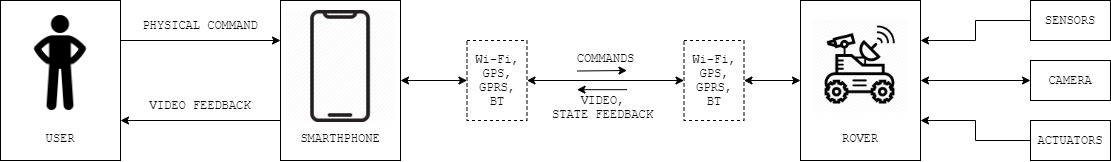
\includegraphics[width=1.0\textwidth]{./sec/img/initial-design.png}
\caption{\label{fig:initial-design}Initial design: Block diagram view}
\end{figure}

Thus, summarising, the initial design yields the system illustrated in
fig.~\ref{fig:initial-design}, comprised of:
\begin{itemize}
\item \textbf{DC Motor}: the prototype provides a moving platform with a conveyor
belt driven by a direct current motor (\emph{Actuation Transducer});
\item \textbf{Controller}: generates the command variable (\emph{Manipulated Voltage})
according to its control rule, in this case, by taking the \emph{Measured
Voltage} as input;
\item \textbf{Generator}: the generator allows us to measure a voltage (electrical
representation of its speed [rpm] --- \emph{Measured Voltage}) that will
later be converted to an estimated speed value;
\item \textbf{Amplifier}: with the \emph{Manipulated Voltage} as input the amplifier
generates an output voltage (\emph{Command Voltage}) that powers the
\emph{Actuation Transducer} (motor);
\item \textbf{Power Source}: powers the DC motor, the user has two options: using
any DC power supply that satisfies the motor power needs or using the
default battery power supply existing in the prototype;
\item \textbf{HMI}: a human-machine interface that allows the user to choose a
specific velocity magnitude and conveyor direction. Some LEDs will be
used later on to inform the user about the current charge of the
battery supply.
\end{itemize}

%%% Local Variables:
%%% mode: latex
%%% TeX-master: "../Phase1"
%%% End:
